\newcommand{\gausssanspts}{
  % (xi,eta) reference element is square with half-width 1
  \draw[->,very thin] (-1.2,0.0) -- (1.2,0.0) node[below] {\small $\xi$};
  \draw[->,very thin] (0.0,-1.2) -- (0.0,1.2) node[left] {\small $\eta$};
  \draw[line width=1.5pt] (1.0,1.0) -- (-1.0,1.0) -- (-1.0,-1.0) -- (1.0,-1.0) -- cycle;
}

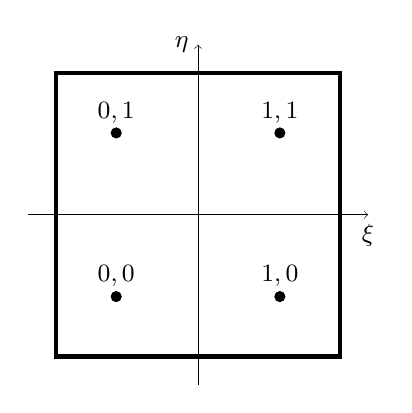
\begin{tikzpicture}[scale=1.8]
\gausssanspts
\pgfmathsetmacro\gl{1.0/sqrt(3.0)}
\foreach \x [count=\RR from 0] in {-\gl,\gl} {
    \foreach \y [count=\SS from 0] in {-\gl,\gl} {
         \filldraw (\x,\y) circle (1.0pt) node[above] {\small $\RR,\SS$};
    }
}
\end{tikzpicture}
\qquad\qquad
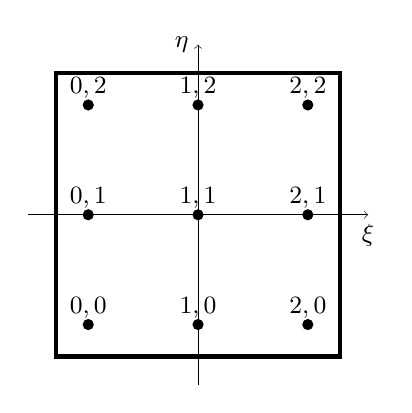
\begin{tikzpicture}[scale=1.8]
\gausssanspts
\pgfmathsetmacro\gl{sqrt(3.0/5.0)}
\foreach \x [count=\RR from 0] in {-\gl,0,\gl} {
    \foreach \y [count=\SS from 0] in {-\gl,0,\gl} {
         \filldraw (\x,\y) circle (1.0pt) node[above,yshift=-0.4mm] {\small $\RR,\SS$};
    }
}
\end{tikzpicture}

